%!TEX root = ../DissertationDefensePresentation.tex

%%--------------------------------------------------------------------------------------------

\subsection{Standard Model}

%%--------------------------------------------------------------------------------------------

\begin{frame}[fragile]
	\tikzstyle{myarrows}=[line width=1mm,draw=magenta,-triangle 45,postaction={draw, line width=3mm, shorten >=4mm, -}]
	\frametitle{The Standard Model: Particle Physics In A Nutshell}
	\vspace*{-0.24cm}
	\begin{block}{}
		\begin{columns}[t,onlytextwidth]
			\column{0.52\textwidth}
			\vspace*{-0.20cm}
			\begin{itemize}
				\small
				\item $SU(3)_{C}{\otimes}SU(2)_{L}{\otimes}U(1)_{Y}$ gauge theory
				\item Forces are mediated by spin-1 gauge bosons (4).
				\begin{itemize}
					\item $\gamma$\enspace- electromagnetic interactions
					\item \Wpm/\cPZ\enspace- weak interactions
					\item \cPg\enspace- strong interactions
				\end{itemize}
			\end{itemize}
			\column{0.51\textwidth}
			\begin{itemize}
				\vspace*{-0.20cm}
				\small
				\item Matter is made up of spin-1/2 fermions
				\begin{itemize}
					\item Leptons (6) and quarks (6)
				\end{itemize}
				\item Spin-0 \textbf{Higgs boson}
				\begin{itemize}
					\item Responsible for the mass of the fundamental particles
				\end{itemize}
			\end{itemize}
		\end{columns}
	\end{block}
	\vspace*{-0.6cm}
	\begin{columns}[T]
		\begin{column}{0.75\textwidth}
	\begin{figure}
		\resizebox{0.82\textwidth}{!}{\input{StandardModel_CERNWebfest2012}}
		\label{fig:standard_model}
	\end{figure}
		\end{column}
		\begin{column}{0.25\textwidth}
			\vspace*{3.75cm}
			Explains \textbf{many} of the properties of the known universe, but not all of them
		\end{column}
	\end{columns}
	\begin{textblock}{0.01}(0.575,0.555)
		\tikz[baseline,remember picture]{\node[coordinate] (t1) {};}
	\end{textblock}
	\begin{textblock}{0.2}(0.75,0.53)
		\tikz[remember picture]{\node[coordinate] (n1) {};}Observation announced July 4th, 2012
		\begin{tikzpicture}[remember picture,overlay]   %% use here too
        	%\path[draw=magenta,thick,->] (n1.west) to (t1.east);
        	\path[myarrows] ([xshift=-2mm]n1.west) to (t1.east);
		\end{tikzpicture}
	\end{textblock}
\end{frame}

\begin{frame}
	\frametitle{Physics Beyond the Standard Model (BSM)}
	\vspace*{-0.24cm}
	%\begin{block}{Why mention BSM?}
	\begin{block}{What is the SM lacking?}
		\begin{itemize}
			\item A dark matter candidate
			\item A way to explain non-zero neutrino mass and neutrino oscillations
			\item A theory of gravity
			\item An explanation for the matter-antimatter asymmetry of the universe
		\end{itemize}
	\end{block}
	\vspace*{-0.15cm}
	\begin{figure}
		\label{fig:BSM}
		\centering
		\begin{subfigure}[t]{0.20\textwidth}
			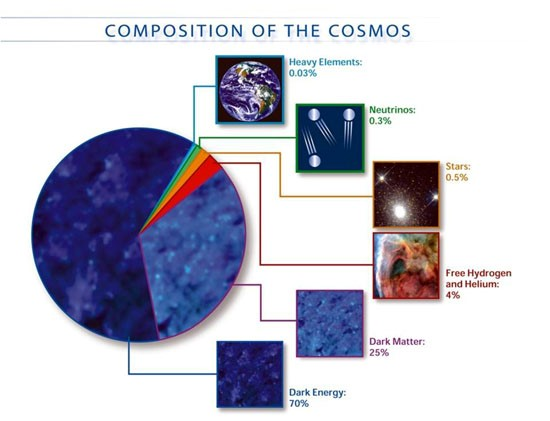
\includegraphics[width=\textwidth]{\figpath/CosmicComposition.jpg}
			\label{fig:BSM1}
		\end{subfigure}
		\hfill
		\begin{subfigure}[t]{0.21\textwidth}
			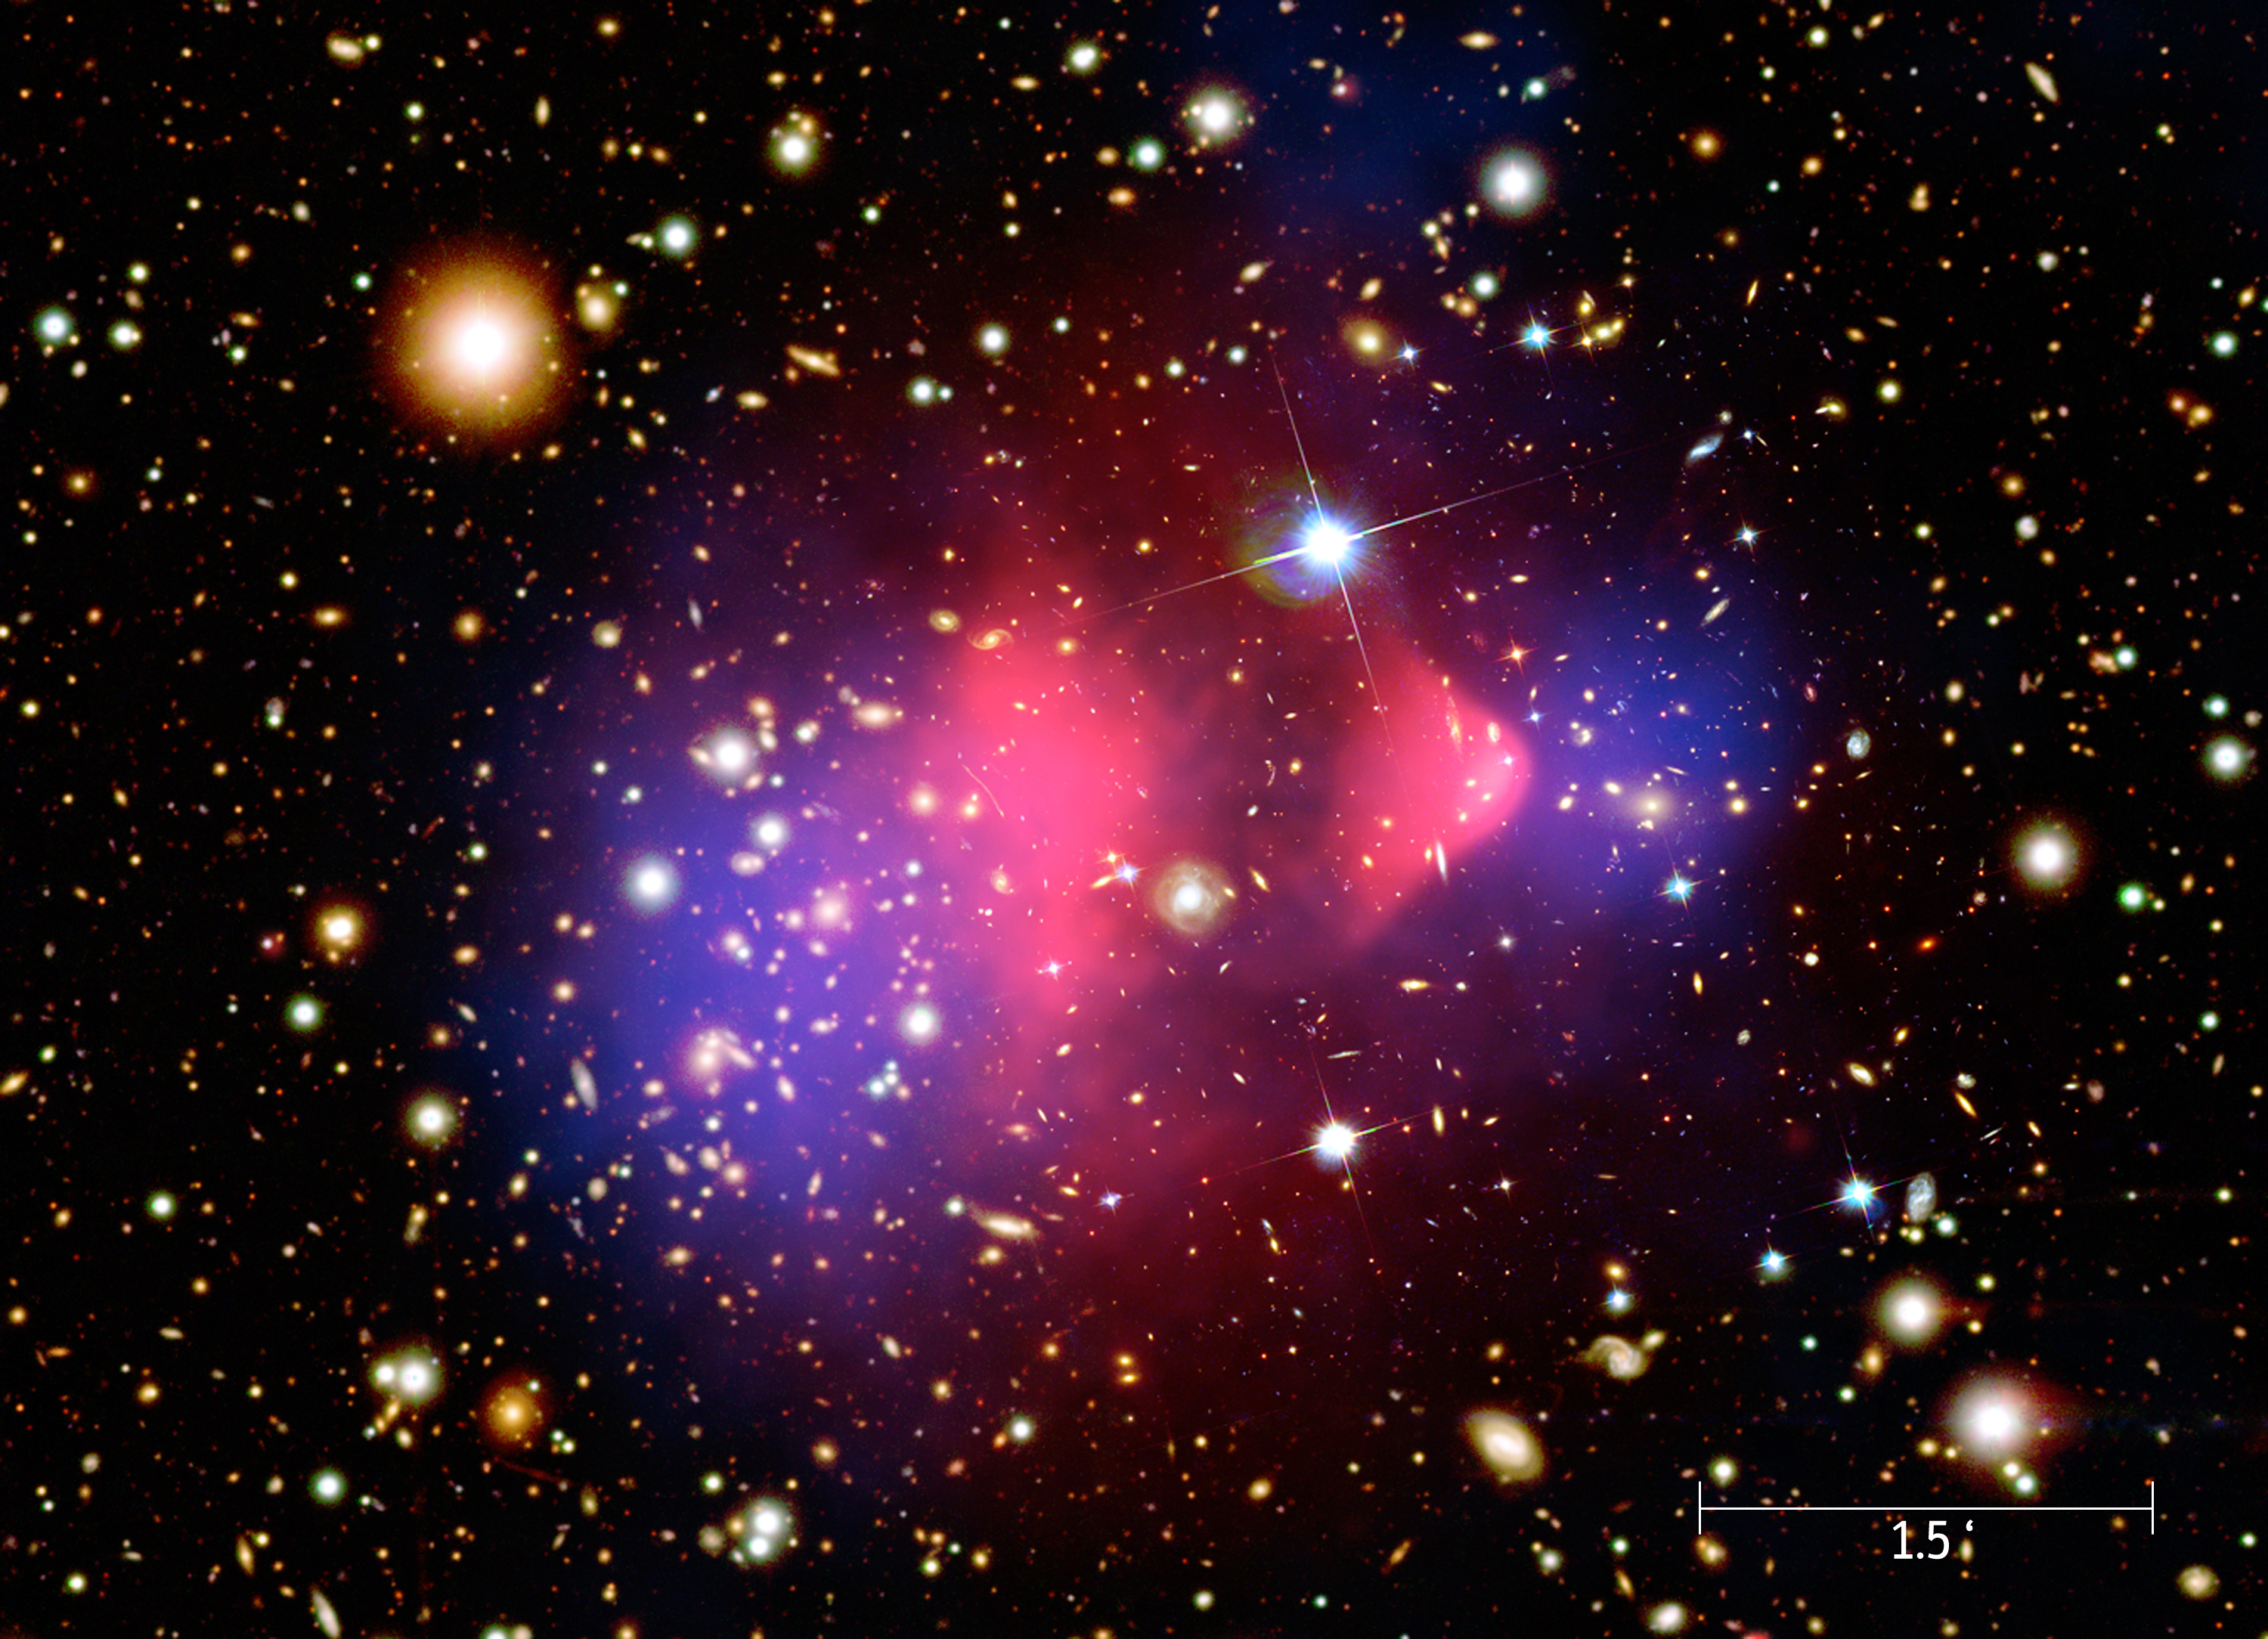
\includegraphics[width=\textwidth]{\figpath/bullet_clusters.jpg}
			\label{fig:BSM2}
		\end{subfigure}
		\hfill
		\begin{subfigure}[t]{0.20\textwidth}
			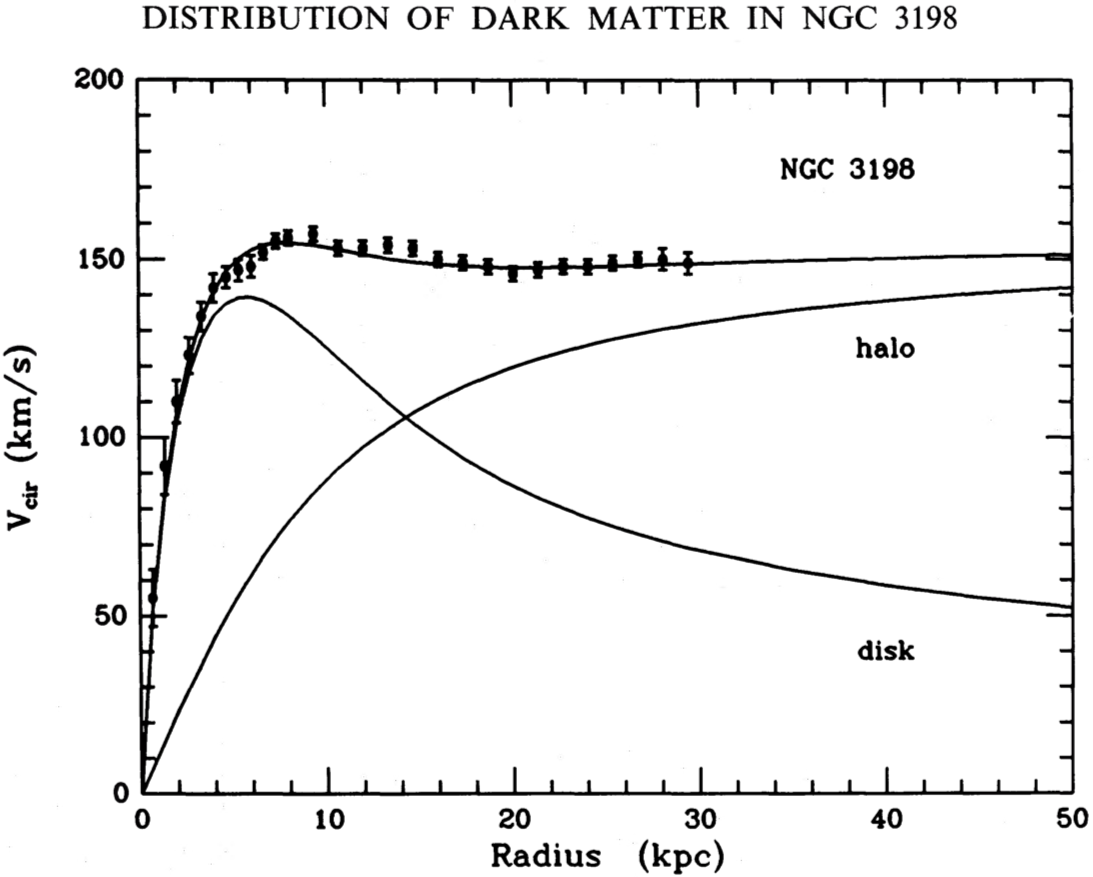
\includegraphics[width=\textwidth]{\figpath/GalaxyHalo.png}
			\label{fig:BSM3}
		\end{subfigure}
		\hfill
		\begin{subfigure}[t]{0.24\textwidth}
			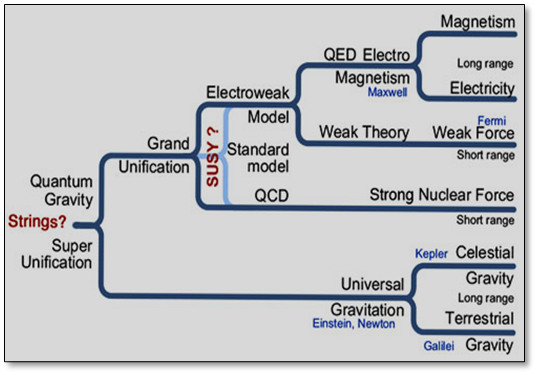
\includegraphics[width=\textwidth]{\figpath/unification.png}
			\label{fig:BSM4}
		\end{subfigure}
	\end{figure}
	\vspace*{-0.30cm}
	\begin{block}{What does Higgs physics have to do with BSM?}
		\begin{itemize}
			\item Need at least one (SM Higgs) to provide mass to particles
			\begin{itemize}
				\item Study the properties of SM Higgs boson, especially its couplings
			\end{itemize}
			\item Additional particles in the Higgs sector at the $\mathcal{O}\left(1 TeV\right)$ scale would be proof of BSM physics
			\begin{itemize}
				\item Could disambiguate supersymmetry (SUSY), from composite Higgs models, etc.
			\end{itemize}
			%\item If we have really observed ``the'' standard model Higgs boson, then we should be able to find it in all decay channels
			%\item If it's not there ($l{\nu}jj$), then either the model is again defficient or we didn't observe the boson we thought we had
			%\item So we must either search for or set limits on the Higgs SM branching ratios
		\end{itemize}
	\end{block}
\end{frame}

\begin{frame}
	\tikzstyle{na} = [baseline=-.5ex]
	\frametitle{Higgs Production}
	\vspace*{-0.8cm}
	\begin{center}
		\begin{tikzpicture}[remember picture]%,show background grid]
            % Put the graphic inside a node. This makes it easy to place the
            % graphic and to draw on top of it. 
            % The above right option is used to place the lower left corner
            % of the image at the (0,0) coordinate. 
            \node [inner sep=0pt,above right] 
                {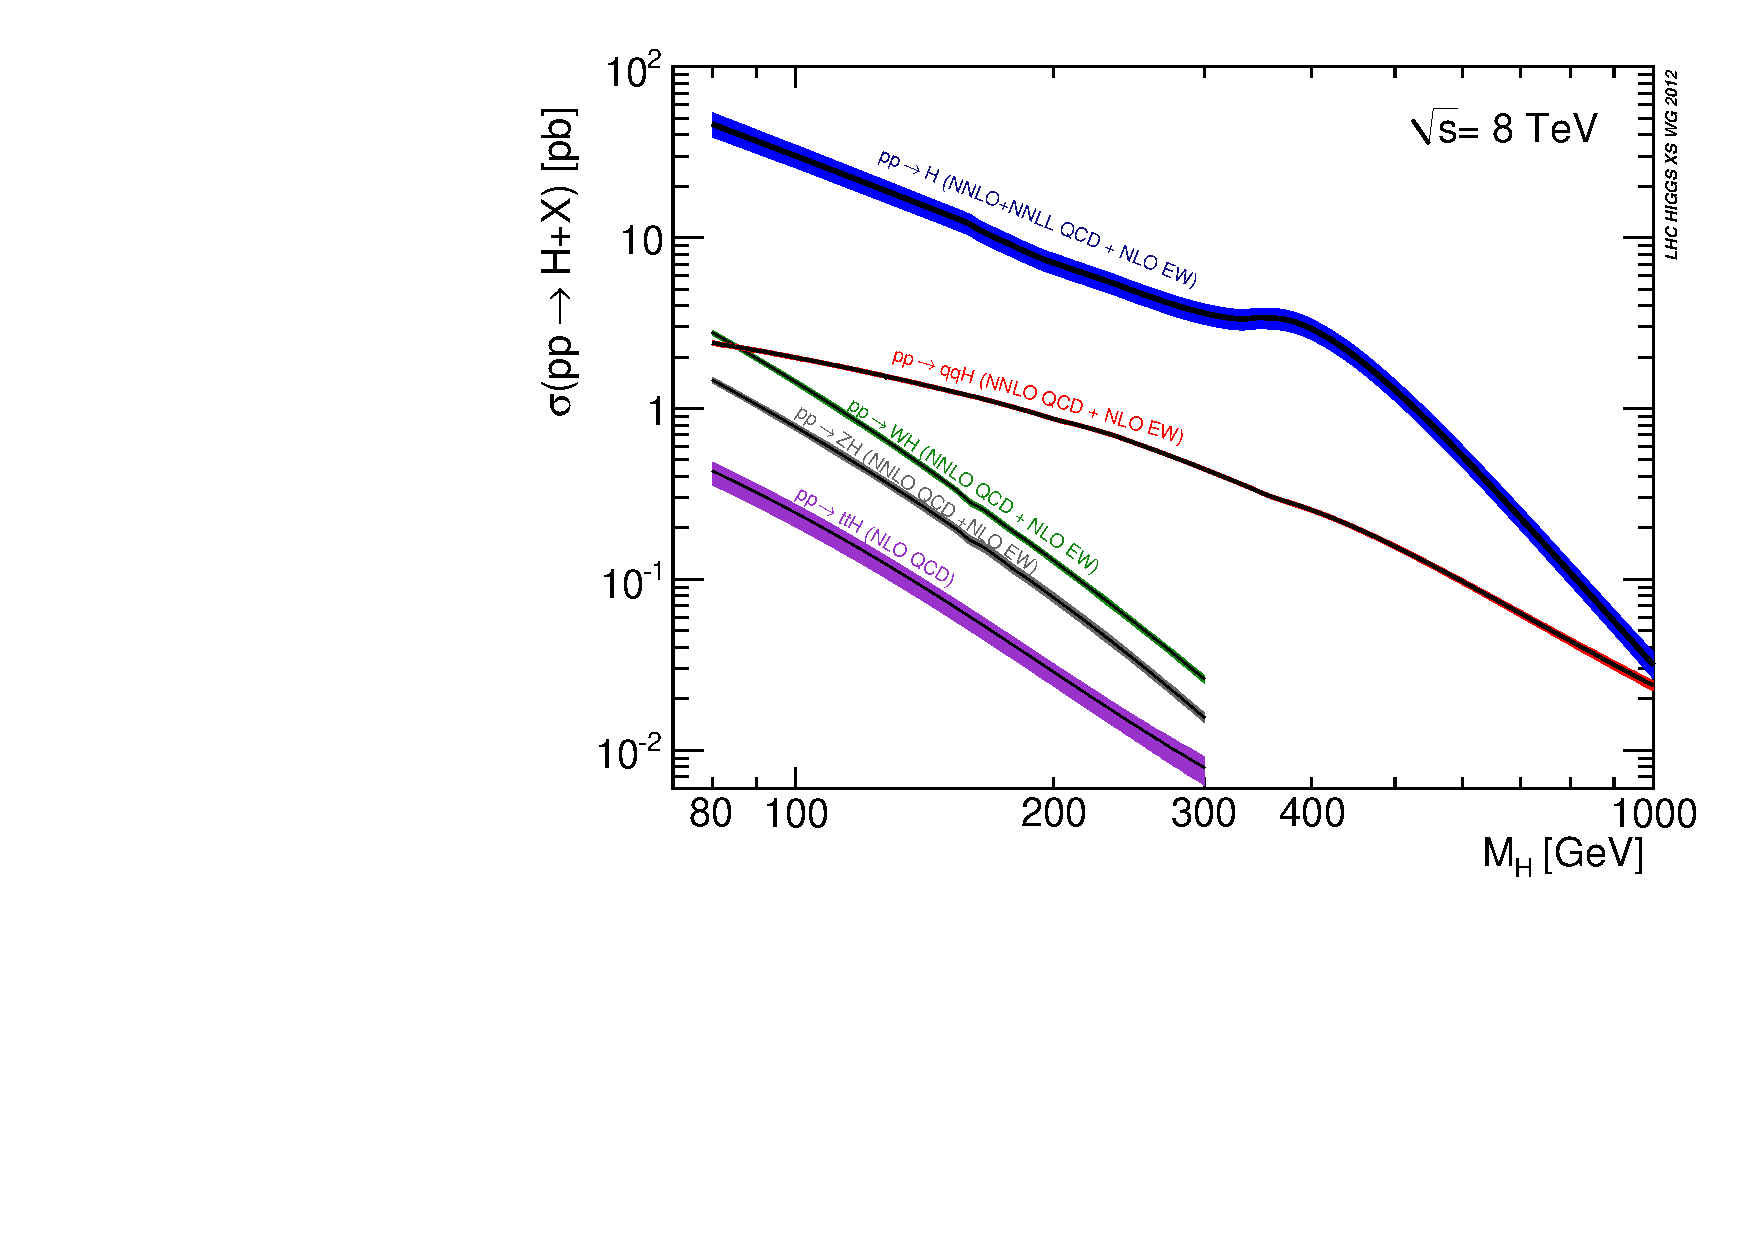
\includegraphics[width=0.65\textwidth]{\figpath/Higgs_XS_8TeV_lx.pdf}};
            % show origin
            \fill (0,0) circle (2pt);
            % define destination coordinates
            \path (6.3,3.2) coordinate (ggH)
                  (6.2,2.0) coordinate (qqH)
                  (1.5,3.5) coordinate (WH)
                  (3.0,1.6) coordinate (ttH);
        \end{tikzpicture}
	\end{center}
	\vfill

	\begin{textblock}{0.24}(0.74,0.32)
		\begin{tcolorbox}[colframe=blue,colback=blue!20!white]
			\tikz[remember picture, na] \coordinate (s-ggH);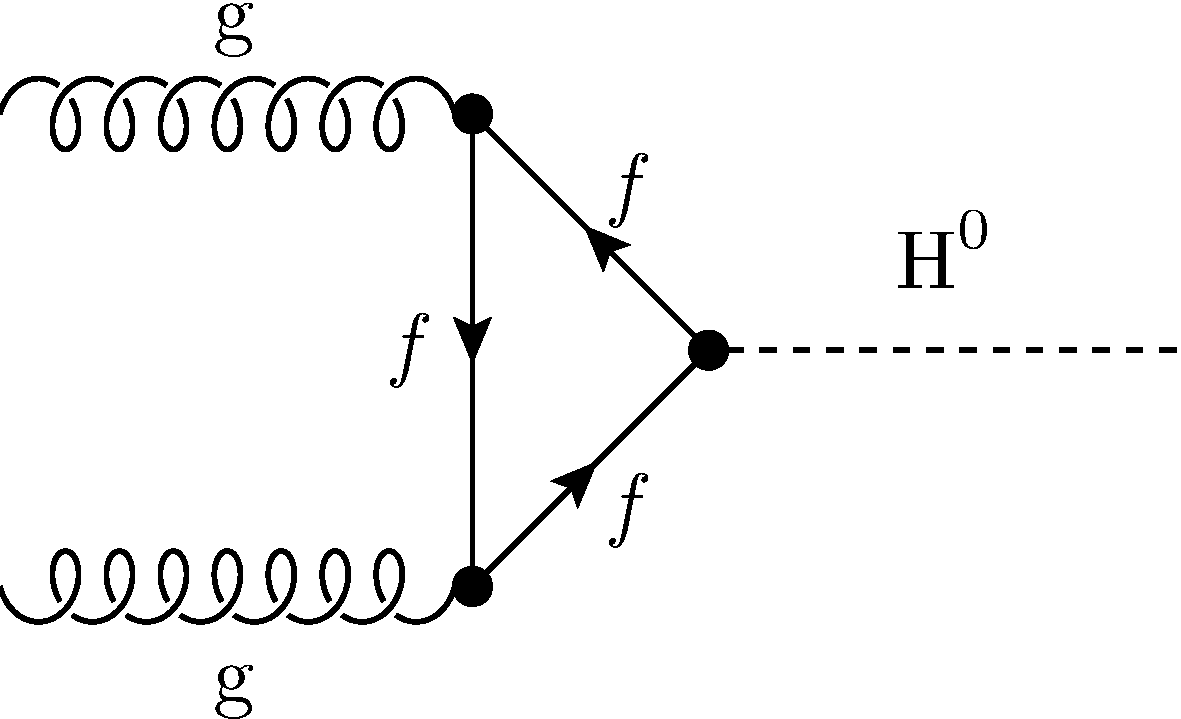
\includegraphics[width=\textwidth]{\figpath/FeynmanDiagrams/ggH.pdf}
			%\tiny \HWW
		\end{tcolorbox}
	\end{textblock}
	\begin{textblock}{0.24}(0.55,0.75)
		\begin{tcolorbox}[colframe=red,colback=red!20!white]
			\tikz[remember picture, na] \coordinate (s-qqH);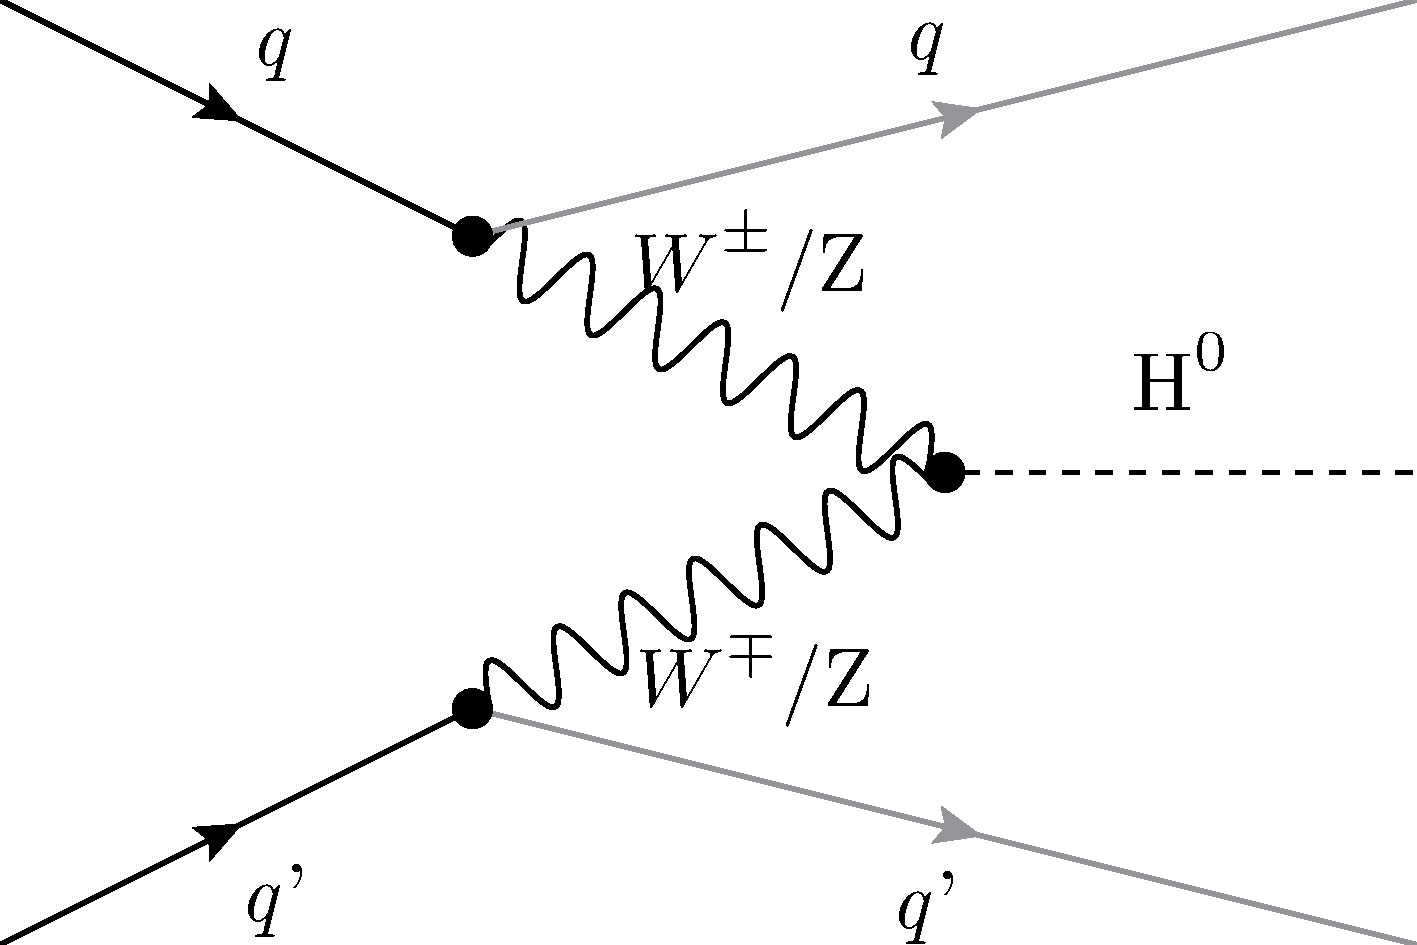
\includegraphics[width=\textwidth]{\figpath/FeynmanDiagrams/qqH.pdf}
			%\tiny \HWW
		\end{tcolorbox}
	\end{textblock}
	\begin{textblock}{0.24}(0.005,0.46)
		\begin{tcolorbox}[colframe=green,colback=green!20!white]
			\tikz[remember picture, na] \coordinate (s-WH);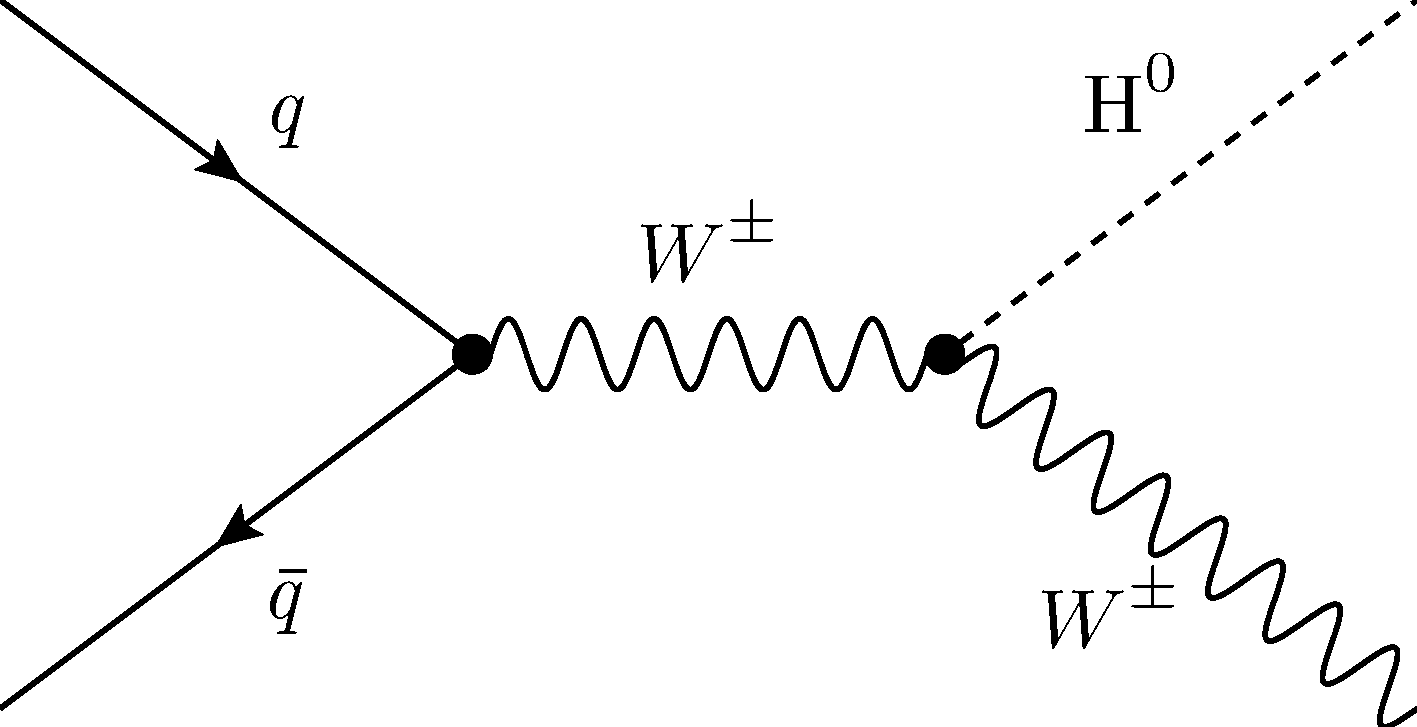
\includegraphics[width=\textwidth]{\figpath/FeynmanDiagrams/WH.pdf}
			%\tiny \HWW, \HZZ, \Hbb (\Wlv)
		\end{tcolorbox}
	\end{textblock}
	\begin{textblock}{0.24}(0.005,0.73)
		\begin{tcolorbox}[colframe=violet,colback=violet!20!white]
			\tikz[remember picture, na] \coordinate (s-ttH);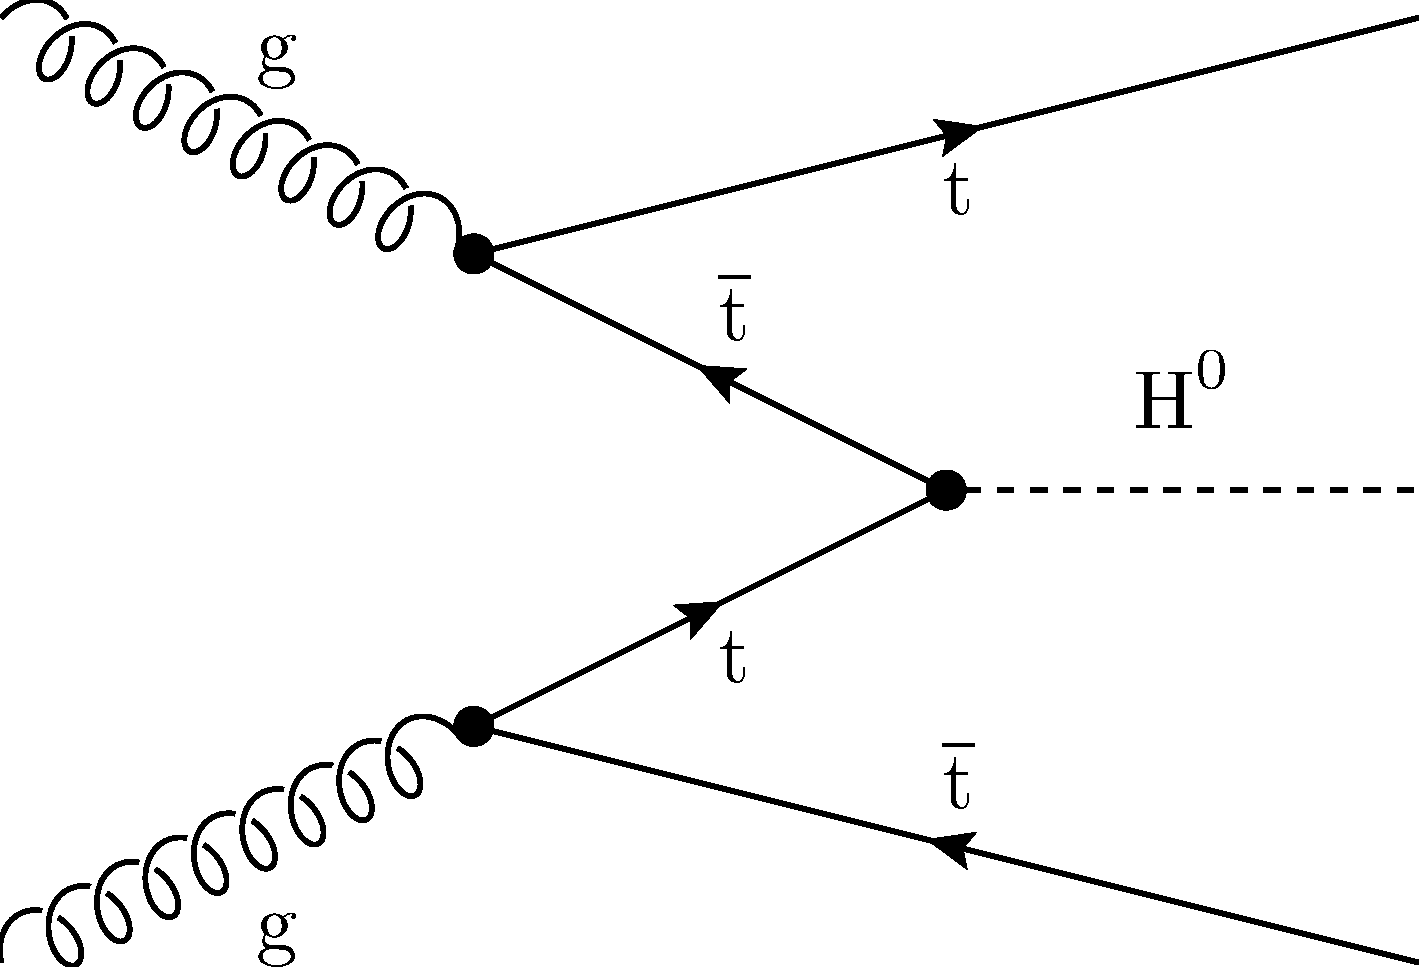
\includegraphics[width=\textwidth]{\figpath/FeynmanDiagrams/ttH.pdf}
			%\tiny \HWW, \HZZ, \Hbb
		\end{tcolorbox}
	\end{textblock}

	\begin{textblock}{0.24}(0.745,0.49)
		\tiny Gluon-Gluon Fusion
	\end{textblock}
	\begin{textblock}{0.24}(0.555,0.93)
		\tiny Vector-Boson Fusion
	\end{textblock}
	\begin{textblock}{0.24}(0.01,0.61)
		\tiny Associated Production
	\end{textblock}
	\begin{textblock}{0.24}(0.01,0.91)
		\tiny \ttbar Fusion
	\end{textblock}
	
	% define overlays
	% Note the use of the overlay option. This is required when 
	% you want to access nodes in different pictures.
	\begin{tikzpicture}[remember picture,overlay]
	        \path[->,blue,thick] ([yshift=5mm]s-ggH) edge (ggH);
	        \path[->,red,thick] ([xshift=1.9cm]s-qqH) edge [bend left] (qqH);
	        \path[->,green,thick] ([yshift=5mm]s-WH) edge [bend right] (WH);
	        \path[->,violet,thick] (s-ttH) edge [out=0, in=-90] (ttH);
	\end{tikzpicture}
\end{frame}

%%--------------------------------------------------------------------------------------------

\subsection[Motivation]{Motivation}

%%--------------------------------------------------------------------------------------------

\begin{frame}
	\frametitle{Higgs Decay}
	\framesubtitle{\small Why search for the Higgs boson in the \HWWlvjj channel?}
	\vspace*{-0.24cm}	
	\begin{columns}[T]
		\column{0.64\textwidth}
			\vspace*{-0.25cm}
			\begin{block}{}
				\begin{itemize}
					\item \HWW analyses:
					\begin{itemize}
						\item Probe the \HWW vertex directly
						\item One of the highest branching ratios
					\end{itemize}
					\item Fully-leptonic analysis (\HWWlvlv)
					\begin{itemize}
						\item Only channel to probe vertex, so far ($\sim$4$\sigma$ result)
						\item Would be nice to have another handle to probe this vertex
					\end{itemize}
					\item \textbf{Semi-leptonic analysis} (\HWWlvjj)
					\begin{itemize}
						\item The good:
						\begin{itemize}
							\item High $\sigma\times$BR for $\MH\sim$125\GeV
							\item Has a reconstructible Higgs boson mass peak
						\end{itemize}
						\item The bad:
						\begin{itemize}
							\item Looked at only for $\MH>\text{2}\MW$
							%\item Searching in the WW channel requires one W to be off-shell since $M_{H}<2M_{W}$
							\item Small signal to background ratio
							%\item The resolution in the semileptonic channel is not as good as the fully-leptonic channel due to the presence of jets and MET
						\end{itemize}
						\item New techniques may make this channel feasible and useful for measuring the properties of the Higgs boson
					\end{itemize}
				\end{itemize}
			\end{block}
		\column{0.015\textwidth}
		\column{0.33\textwidth}
			\vspace*{-0.33cm}
			\begin{myfancyblock}
				\node[anchor=south west,inner sep=0] (image) at (0,0) {%
					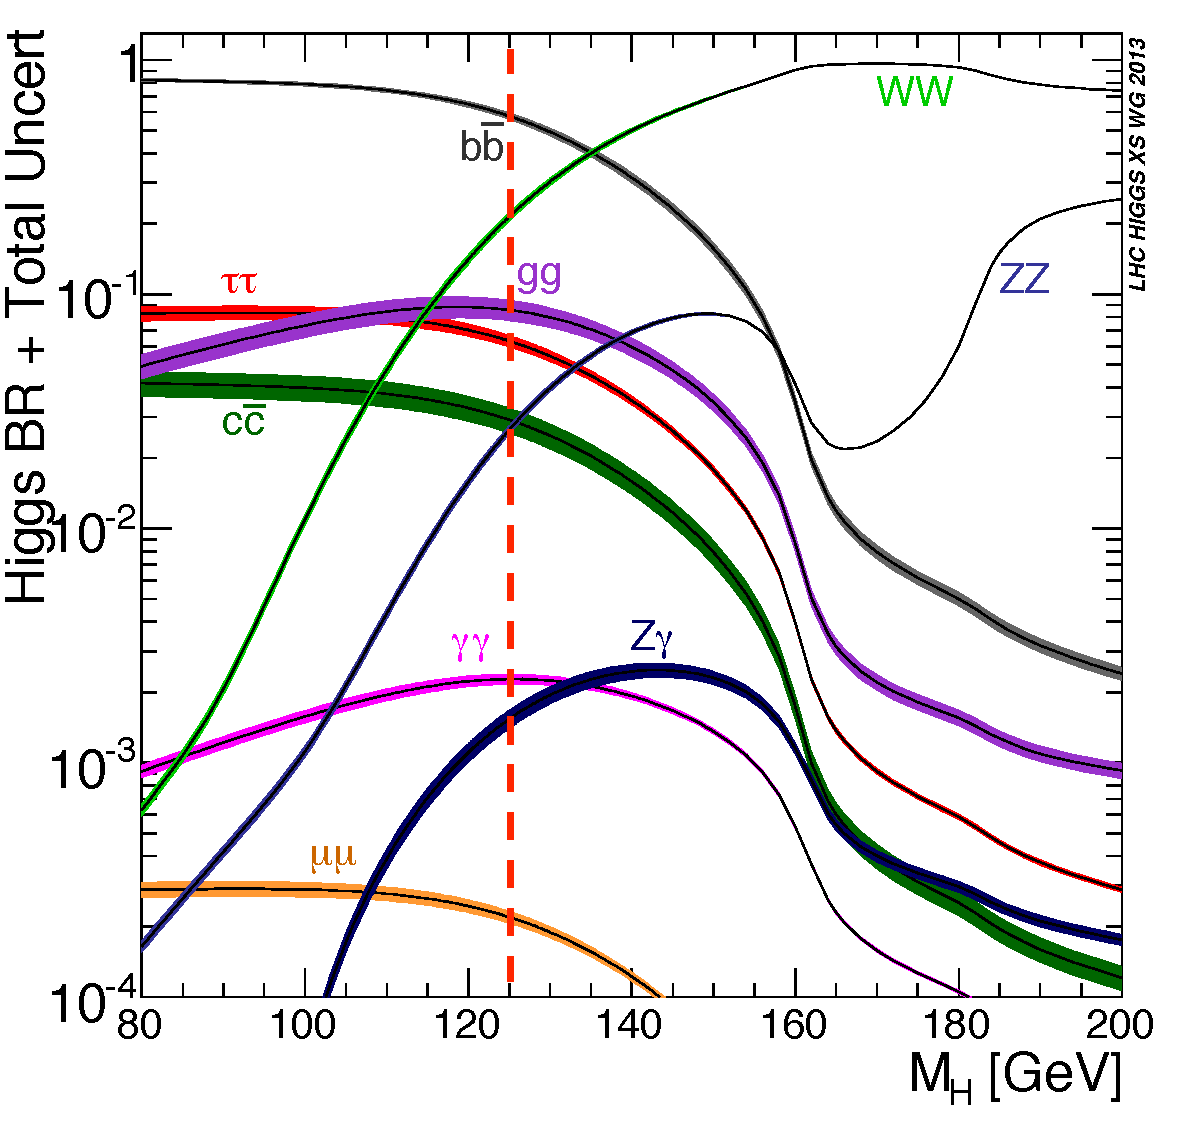
\includegraphics[width=\textwidth]{\figpath/Higgs_BR_LM.pdf}
				};
				\node[anchor=south west,inner sep=0] (image2) at (0,-3.9) {%
					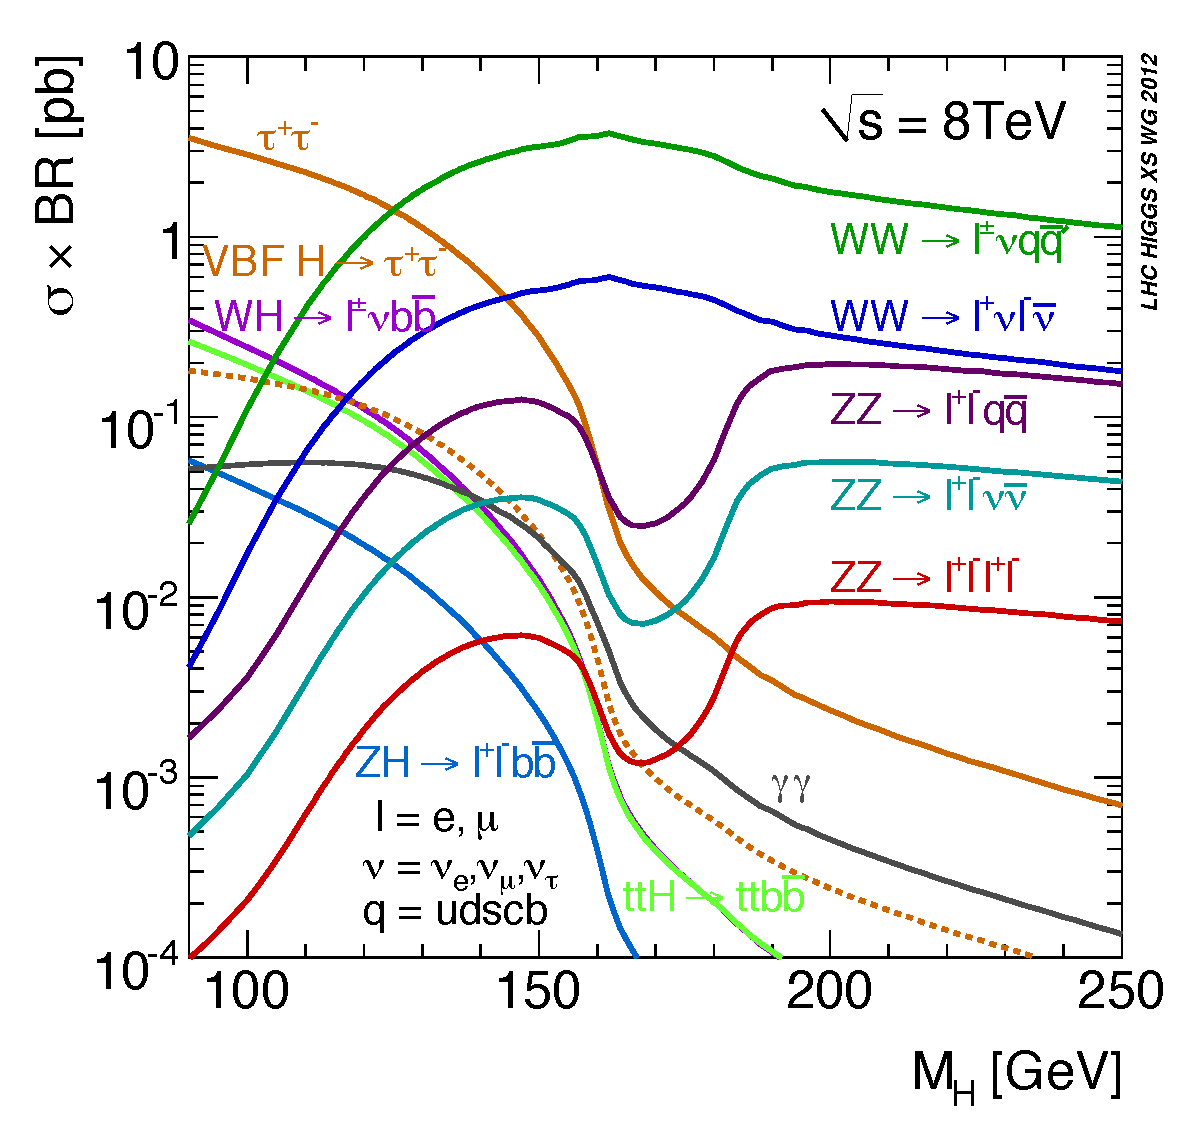
\includegraphics[width=\textwidth]{\figpath/XSBR_8TeV_SM_LM}
				};
				\draw[orange,thick] (1.755,3.78) -- (1.755,0.465);
				\draw[orange,thick] (1.38,-0.17) -- (1.38,-3.27);
			\end{myfancyblock}

			%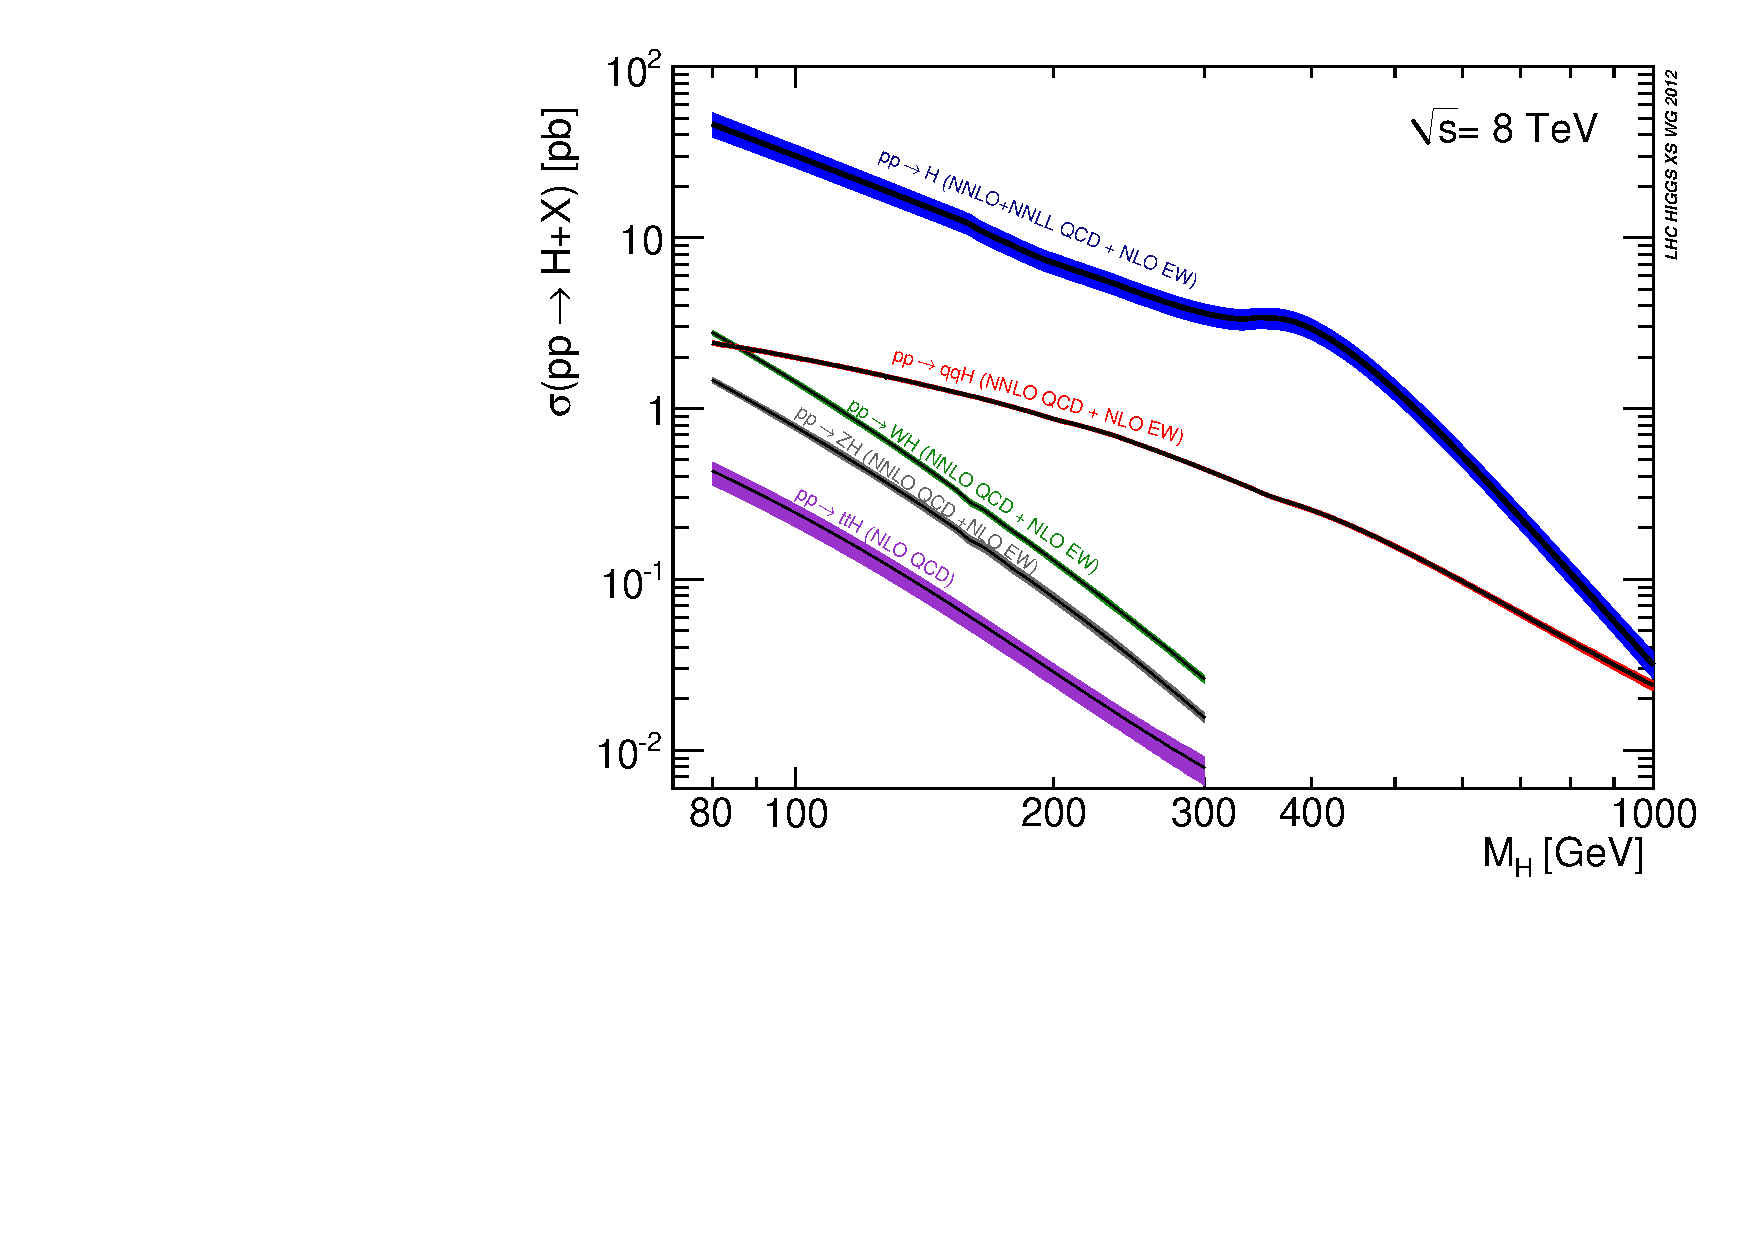
\includegraphics[width=\textwidth]{\figpath/Higgs_XS_8TeV_lx.pdf}\\
			%\vspace*{-0.1cm}
			%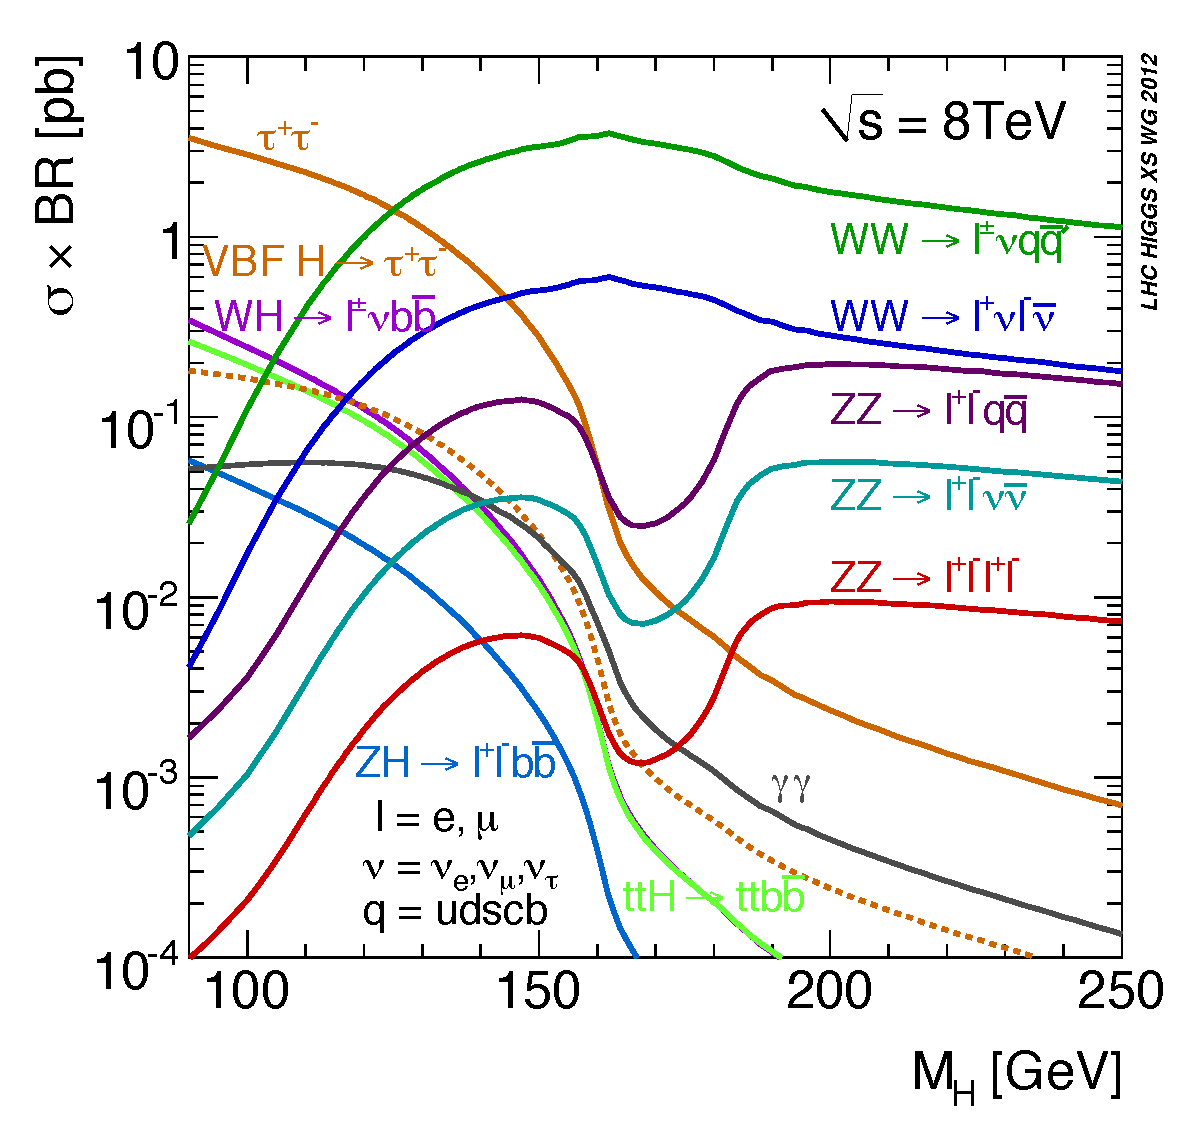
\includegraphics[width=\textwidth]{\figpath/XSBR_8TeV_SM_LM}
	\end{columns}
\end{frame}
